\documentclass[portuguese, conference]{IEEEtran}
\usepackage{blindtext, graphicx, pgfplots}
\graphicspath{{images/}}

\usepackage[utf8]{inputenc}
\usepackage[round]{natbib}
\usepackage[T1]{fontenc}
\usepackage{lmodern} % load a font with all the characters
\usepackage[]{algorithm2e}

% correct bad hyphenation here
\hyphenation{op-tical net-works semi-conduc-tor}

\begin{document}
\title{Programação Paralela: Paradígma Mestre-Escravo}

% author names and affiliations
% use a multiple column layout for up to three different
% affiliations
\author{\IEEEauthorblockN{Filipe Franciel Utzig}
\IEEEauthorblockA{Engenharia de Computação\\
PUC-RS\\
Porto Alegre 90619-900
\\
Email: filipeutzig \textit{at} gmail.com}}

% make the title area
\maketitle

\begin{abstract}
\it{The present work implements the sorting algorithm known as Rank Sort. The algorithm will be implemented in two forms: parallel, using openMPI library with the master/slave paradigm, and sequential, so that, at the end, we can have a better knowledge regarding the performance and efficiency of the parallel version.}
\end{abstract}

% Note that keywords are not normally used for peerreview papers.
\begin{IEEEkeywords}
MPI; Rank-Sort; parallelism;
\end{IEEEkeywords}

\IEEEpeerreviewmaketitle

\section{Descrição do problema}

Dado um vetor desordenado, para cada elemento \textit {x} desse vetor, conta-se o número de elementos que são menores que o mesmo. Este número será o índice de \textit{x} no vetor ordenado. O procedimento é repetido para todos os valores da lista. O algoritmo com que estamos trabalhando não aceita um vetor com possíveis repetições de valores.

\section{Atacando o problema}

O {\it Rank Sort}~\cite{JOH15}~\cite{BEA15} tem o seu funcionamento sequencial descrito no Algoritmo~\ref{Rank_sort}, onde é verificado a quantidade de valores que são menores que o valor selecionado, esta contagem provê a posição no vetor ordenado.

\begin{algorithm}[]
\label{Rank_sort}
    \For{(i=0; i < n; i++)}{
        \For{(j=0; j < n; j++)}{
            \If{(a[i]>a[j])}{
                x++\;
            }
        }
         b[x] = a[i]\;
    }
    
 \caption{{\it Rank Sort} sequencial}
\end{algorithm}

Como é possível notar, o algoritmo {\it Rank Sort} é de ordem O($n^{2}$), para cada elemento adicional no vetor o tempo de execução cresce de forma quadrática. Para implementar o Algoritmo~\ref{Rank_sort} foi utilizado a linguagem programação C e, na versão paralela deste, a biblioteca openMPI~\cite{HAM13}, rodando sobre o sistema operacional Linux.

\subsection{Descrição da Implementação Sequencial}
A implementação sequencial espera receber como entrada o caminho para um arquivo contendo os valores embaralhados e o número de elementos a serem ordenados. Ao começar programa é feita a leitura de todos valores para um vetor alocado em memória, evitando assim que chamadas de sistemas sejam executadas durante a medição de tempo do algoritmo.

Essa versão ordena o vetor inteiro de uma vez só. Para cada elemento \textit{Y} do vetor, o algoritmo simplesmente guarda numa variável \textit{x}, o numero de elementos que são menores do que \textit{Y}, feita essa comparação, o programa coloca o elemento \textit{Y} na posição \textit{x}. Esse laço é executado para cada elemento do vetor, o resultado ao final é o vetor ordenado de forma crescente, que é escrito num arquivo texto ao final da execução.

\subsection{Descrição da Implementação Paralela}

O funcionamento da implementação paralela segue a mesma lógica da versão sequencial, porém é necessária uma logica de controle de paralelismo e divisão de tarefas.

No início da execução o Mestre divide o vetor desordenado em diversos pedaços, que serão mandados para os Escravos. O número de elementos que cada escravo recebe é dado por \textit{\textbf{N/4*M}} onde \textbf{N} é igual ao número total de elementos do vetor desordenado e \textbf{M} equivale ao número de escravos que executarão a tarefa.

Inicialmente, o Mestre atribui um pedaço do vetor desordenado para cada escravo. Como o número de pedaços é maior que o número de escravos, o processo Mestre fica aguardando um Escravo terminar de ordenar o pedaço que lhe foi atribuído. Quando o primeiro escravo termina o seu ordenamento, ele o envia o resultado parcial ao mestre, que o recebe e envia um novo pedaço à esse escravo. A cada fatia recebida pelo Mestre, uma sub-rotina concatena de forma ordenada dos pedaços recebidos. Esse processo é repetido até que não haja mais pedaços a serem enviados. 

\section{Resultados}

Todos os testes foram executados no {\it cluster} Amazônia que consiste em uma  {\it enclosure} HP BladeSystem C3000 com 4 Blades BL620c G7 e uma {\it storage} dedicada com acesso via Fiber Channel Protocol(8 Gib/s). Cada máquina possui dois processadores Intel Xeon E7 - 2850 2.0 GHz Hyper-Threading e 80GB de memória, totalizando 20 núcleos (40 {\it threads}) por nó e 80 núcleos (160 {\it threads}) no {\it cluster}. Os nós estão interligados por 4 redes {\it Gigabit-Ethernet} chaveadas e 2 redes InfiniBand (para comunicação entre os nós)~\cite{IDE15}. 

A Tabela~\ref{tab1} contém os tempos de execução dos testes, cada teste foi executado 3 vezes a fim de aumentar a confiabilidade dos dados adquiridos, e os resultados apresentados é a média simples das execuções. Podemos observar um decréscimo de tempo em todos os casos com a paralelização dos processos, inclusive quando somente um escravo realiza a tarefa, esse comportamento ocorre pois o escravo ordena uma fatia 4x menor por vez, não percorrendo toda a extensão do vetor e devido a complexidade quadrática do algoritmo fica explicado os resultados vantajosos. Podemos observar melhor esse comportamento através da Figura ~\ref{fig:tempo}.

\begin{figure}[htb]
\raggedright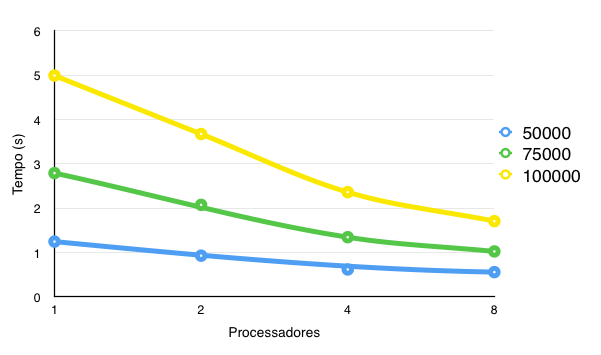
\includegraphics[width=.5\textwidth]{tempo.png}
\caption{\label{fig:tempo} Tempo de execução dos testes em função do número de elementos do vetor.}
\end{figure}

\begin{table}[h]
\centering
\caption{Tempo de Execução dos testes.}
\label{tab1}
\begin{tabular}{|c|c|c|c|}
\hline
\begin{tabular}[c]{@{}c@{}}Número de\\ Processadores\end{tabular} & \begin{tabular}[c]{@{}c@{}}50000\\ Elementos\end{tabular} & \begin{tabular}[c]{@{}c@{}}75000\\ Elementos\end{tabular} & \begin{tabular}[c]{@{}c@{}}100000\\ Elementos\end{tabular} \\ \hline
1               & 3,861 s               & 8,662 s               & 14,632 s              \\ \hline
2               & 1,033 s               & 2,236 s               & 3,997 s               \\ \hline
4               & 0,176 s               & 0,318 s               & 0,514 s               \\ \hline
8               & 0,039 s               & 0,085 s               & 0,150 s               \\ \hline
\end{tabular}
\end{table}

O aumento na velocidade de execução foi notável, de forma a quantificar o aumento, foi calculado o {\it Speed Up}~\cite{BEA15} de cada teste, que é obtido de acordo com a Equação~\ref{eq:eq1} onde T\textsubscript{s} é o tempo do algoritmo sequencial e T{\textsubscript{n}} é o tempo do algoritmo paralelo, a Tabela~\ref{speed_up} contém todos os valores referentes a {\it Speed Up}, nela podemos observar que nesse caso o desempenho possuí um comportamento super linear, pois $Sp > Np$. Podemos observar o comportamento do {\it Speed Up} através da Figura~\ref{fig:speed}.

\begin{figure}[htb]
\raggedright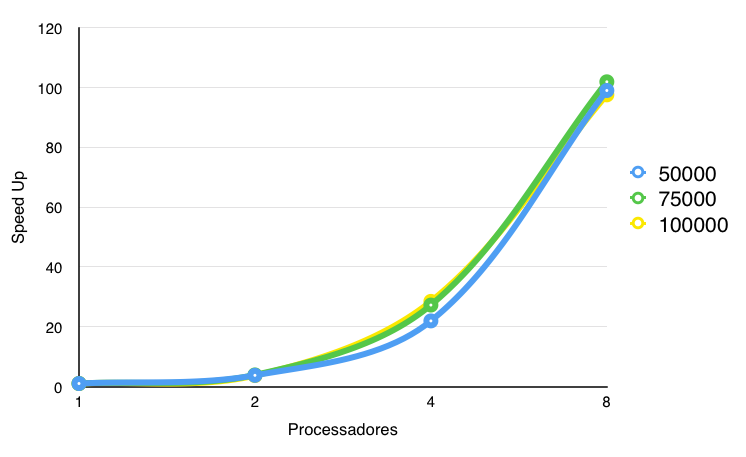
\includegraphics[width=.5\textwidth]{speedup.png}
\caption{\label{fig:speed}Speed up.}
\end{figure}

\begin{equation}\label{eq:eq1}
    SpeedUp = \frac{T\textsubscript{s}}{ T\textsubscript{n}}
\end{equation}

\begin{table}[h]
\centering
\caption{Speed Up dos testes.}
\label{speed_up}
\begin{tabular}{|c|c|c|c|}
\hline
\begin{tabular}[c]{@{}c@{}}Número de\\ Processadores\end{tabular} & \begin{tabular}[c]{@{}c@{}}50000\\ Elementos\end{tabular} & \begin{tabular}[c]{@{}c@{}}75000\\ Elementos\end{tabular} & \begin{tabular}[c]{@{}c@{}}100000\\ Elementos\end{tabular} \\ \hline
1               & 1                     & 1                     & 1                     \\ \hline
2               & 3,74                  & 3,87                  & 3,66                  \\ \hline
4               & 21,94                 & 27,24                 & 28,47                 \\ \hline
8               & 99,00                 & 101,91                & 97,55                 \\ \hline
\end{tabular}
\end{table}

Outro método de aferir o ganho da implementação paralela é através da eficiência, calculada a partir da Equação~\ref{eq:eq2}, todos os dados encontram-se na Tabela~\ref{efic}. Observamos que os casos com 4 e 8 processadores obtiveram um coeficiente de eficiência superior ao número de processadores utilizados, com isto é possível verificar que o desempenho melhora substancialmente na forma paralelizada, e este comportamento se deve à característica da ordem quadrática do algoritmo, no qual quanto menor for o número de elementos processados por cada escravo, muito mais rápida será a execução do ordenamento. O comportamento da eficiência dessa paralelização está ilustrada na Figura~\ref{fig:eficiencia}.

\begin{equation}\label{eq:eq2}
    Eficiência = \frac{SpeedUp}{n}
\end{equation}

\begin{table}[h]
\centering
\caption{Eficiência dos testes.}
\label{efic}
\begin{tabular}{|c|c|c|c|}
\hline
\begin{tabular}[c]{@{}c@{}}Número de\\ Processadores\end{tabular} & \begin{tabular}[c]{@{}c@{}}50000\\ Elementos\end{tabular} & \begin{tabular}[c]{@{}c@{}}75000\\ Elementos\end{tabular} & \begin{tabular}[c]{@{}c@{}}100000\\ Elementos\end{tabular} \\ \hline
1               & 1                     & 1                     & 1                     \\ \hline
2               & 1,87                  & 1,94                  & 1,83                  \\ \hline
4               & 5,48                  & 6,81                  & 7,12                  \\ \hline
8               & 12,38                 & 12,74                 & 12,19                 \\ \hline
\end{tabular}
\end{table}

\begin{figure}[htb]
\raggedright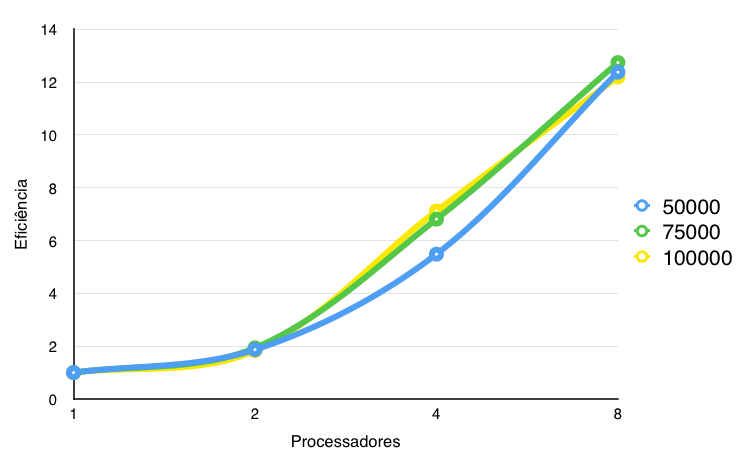
\includegraphics[width=.5\textwidth]{eficiencia.png}
\caption{\label{fig:eficiencia}Eficiência.}
\end{figure}

\section{Conclusão}

Podemos observar que com a paralelização do problema obtivemos um ganho de performance significativo. Nos cenários simulados foi possível verificar que conforme o número de processadores era aumentado o {\it Speed Up} também aumentava, porém esse comportamento não é linear, pois se aumentarmos muito o número de processadores chegaremos um ponto em que o gargalo será a comunicação entre esses diversos escravos.

\bibliographystyle{IEEEtran}
\bibliography{referencia}

\end{document}
